\section{External Evaluation and Failure Analysis}
\label{sec:external}

\paragraph{Setup.} The unchanged pipeline analysed the UCI-498 incident
log~\cite{amaral2018uci498}, a real ServiceNow event log of one organization's IT
service desk, with each final assignment group of sufficient size treated as an
entity: \V{X02b-groups} groups, \V{X02b-incidents} of \V{X02b-incidents-total}
incidents, \V{X02b-events} investigation-step proxies derived from work-state events
and \V{X02b-reassign} escalation proxies derived from reassignments. The only outcome
available is the final SLA flag. SLA labels were loaded only after SAT-SA's ranking
existed and never entered a submission. \emph{This is IT incident data, not SOC data};
it is, however, the log on which prior work demonstrated incident-management
compliance assessment~\cite{palma2024eurova} and modelled SLA
attainment~\cite{swain2022sla}.

\paragraph{Feasibility.} All \V{X02b-rows-received} submitted rows were accepted
(\V{X02b-rows-rejected} rejected) and every group's analysis completed, with a median
of \V{X02b-analysis-median}\,s per group.

\paragraph{Negative result.} SAT-SA's risk $R_e$ was not associated with the SLA-miss
rate: Spearman $\rho=\V{X02b-rho-risk}$, 95\% bootstrap \V{X02b-rho-risk-lo} to
\V{X02b-rho-risk-hi} (Table~\ref{tab:external}, Fig.~\ref{fig:external}). Slowest median
resolution reached $\rho=\V{X02b-rho-slowest}$ (\V{X02b-rho-slowest-lo} to
\V{X02b-rho-slowest-hi}), a strong positive association with the SLA-miss rate,
which is expected because slow resolution and missed resolution deadlines measure
closely related aspects of timeliness; reassignment rate
reached \V{X02b-rho-reassign}. Among the \V{X02b-relevant} groups in the top SLA-miss
quartile, SAT-SA's precision@10\% was \V{X02b-p10-satsa} (random \V{X02b-p10-random},
slowest resolution \V{X02b-p10-slowest}), and it needed to review \V{X02b-volume-satsa}
groups to find all of them (slowest resolution \V{X02b-volume-slowest}).

\begin{table}[!htbp]
\caption{UCI-498 IT incident log (X02b, X03): Spearman association of group scores
with the SLA-miss rate over \V{X02b-groups} assignment groups of one organization
(95\% seeded bootstrap intervals). Not SOC data.}
\label{tab:external}
\centering
\scriptsize
\begin{tabular}{@{}L{6.2cm}rr@{}}
\toprule
Group score & Spearman $\rho$ & 95\% interval \\
\midrule
SAT-SA risk $R_e$ & \V{X02b-rho-risk} & \V{X02b-rho-risk-lo} to \V{X02b-rho-risk-hi} \\
Incident volume & \V{X02b-rho-volume} & \V{X02b-rho-volume-lo} to \V{X02b-rho-volume-hi} \\
Reassignment rate & \V{X02b-rho-reassign} & \V{X02b-rho-reassign-lo} to \V{X02b-rho-reassign-hi} \\
Slowest median resolution (upper reference) & \V{X02b-rho-slowest} & \V{X02b-rho-slowest-lo} to \V{X02b-rho-slowest-hi} \\
\midrule
Execution-gap dimension of $R_e$ (X03) & \V{X03-rho-execgap} & \V{X03-rho-execgap-lo} to \V{X03-rho-execgap-hi} \\
Fast-closure prevalence (X03) & \V{X03-rho-fast} & \V{X03-rho-fast-lo} to \V{X03-rho-fast-hi} \\
\bottomrule
\end{tabular}
\end{table}


\begin{figure}[!htbp]
\centering
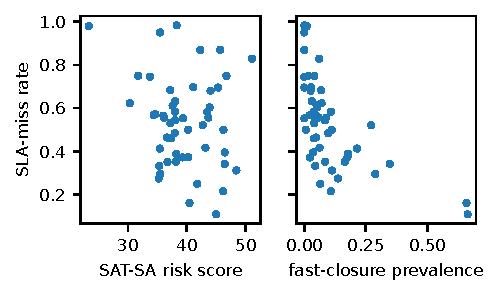
\includegraphics[width=0.78\linewidth]{figures/fig-external.pdf}
\caption{UCI-498 IT incident log (not SOC data): SAT-SA risk (left) and fast-closure
prevalence (right) against the SLA-miss rate; one point per assignment group
(\V{X02b-groups} groups; X02b, X03).}
\label{fig:external}
\end{figure}

\paragraph{Failure analysis.} A diagnostic analysis (X03) on the same data changed no
detector, threshold or weight. It identifies four contributing explanations; the
data are observational and the analysis is diagnostic, not causal.
\emph{(i) Construct mismatch (primary).} On a service desk, fast resolution is the
goal: the prevalence of fast closures was \emph{negatively} associated with SLA misses
($\rho=\V{X03-rho-fast}$, \V{X03-rho-fast-lo} to \V{X03-rho-fast-hi}). SAT-SA treats
fast closure of a security alert as possible skipped investigation, so its execution-gap
dimension, which this signal drives, ran opposite to the outcome
($\rho=\V{X03-rho-execgap}$, \V{X03-rho-execgap-lo} to \V{X03-rho-execgap-hi}). SLA
timeliness and supervisory execution quality are different constructs, and here they
move in opposite directions. \emph{(ii) Detector saturation.} \V{X03-saturated} detector
families fired for every group although their input conditions varied widely---cases
without any step \V{X03-cases-min} to \V{X03-cases-max} of cases, medium-or-higher alerts
with fewer than two steps \V{X03-alerts-min} to \V{X03-alerts-max}. Existence rules
cannot discriminate submissions with thousands of tickets, and Eq.~\eqref{eq:risk}
adds near-constant amounts for them because it ignores prevalence; risk still took
\V{X03-risk-distinct} distinct values and was unrelated to volume
($\rho=\V{X03-risk-vs-volume}$). \emph{(iii) Missing supervisory dimensions.}
\V{X03-zero-dims} of the \V{CODE-dimensions} risk dimensions had no input data;
investigation steps and escalations are proxies (state changes and reassignments), and
monitoring coverage is unavailable. \emph{(iv) A minor adapter artifact.} The log has
no step notes; the adapter submits empty notes, which satisfy a repeated-investigation
rule in \V{X03-note-rule} groups. The analysis found no temporal or label defect: only
\V{X03-other-group} of \V{X03-missed} SLA misses occurred while another group held the
ticket, and reassigned incidents missed more often (\V{X03-reassigned-miss} versus
\V{X03-notreassigned-miss}), consistent with the positive reassignment association.

\paragraph{Decision.} No risk-model change was made. Changing detectors or weights to
raise the correlation with SLA misses would optimize SAT-SA toward a timeliness
construct it is not designed to measure, using the evaluation data for tuning. We
therefore read X02b and X03 as \emph{feasibility and construct-validity evidence}, not
as external validation of effectiveness: on data whose outcome measures a different
construct and that lacks investigation, escalation and coverage semantics, SAT-SA's
supervisory signals did not transfer.
